\documentclass[mathserif,10pt]{beamer}
\usepackage[T1]{fontenc}
\usepackage{amsmath, amssymb}
\usepackage{times}
\usepackage{newtxtext}
\usepackage{algorithm}  
\usepackage{algorithmic} 
\usepackage{caption}
\usepackage{animate} 
\usepackage{lipsum} % just to generate dummy text

\usetheme[
%%% option passed to the outer theme
%    progressstyle=fixedCircCnt,   % fixedCircCnt, movingCircCnt (moving is deault)
  ]{Feather}
  
% If you want to change the colors of the various elements in the theme, edit and uncomment the following lines

% Change the bar colors:
%\setbeamercolor{Feather}{fg=red!20,bg=red}

% Change the color of the structural elements:
%\setbeamercolor{structure}{fg=red}

% Change the frame title text color:
%\setbeamercolor{frametitle}{fg=blue}

% Change the normal text color background:
%\setbeamercolor{normal text}{fg=black,bg=gray!10}

%-------------------------------------------------------
% INCLUDE PACKAGES
%-------------------------------------------------------

\usepackage[utf8]{inputenc}
\usepackage[english]{babel}
\usepackage[T1]{fontenc}
\usepackage{helvet}

%-------------------------------------------------------
% DEFFINING AND REDEFINING COMMANDS
%-------------------------------------------------------

% colored hyperlinks
\newcommand{\chref}[2]{
  \href{#1}{{\usebeamercolor[bg]{Feather}#2}}
}

%-------------------------------------------------------
% INFORMATION IN THE TITLE PAGE
%-------------------------------------------------------

\title[Mathematics in OI] % [] is optional - is placed on the bottom of the sidebar on every slide
{ % is placed on the title page
      \textbf{Mathematics in Olympiad in Informatics \\[0.3cm] Part 2}
}


\author[Haoyue Shi]
{      Frederica Haoyue Shi \\
      {\ttfamily hyshi@pku.edu.cn}
}

\institute[School of EECS, Peking University]
{
      School of Electronics Engineering and Computer Science\\
	  Peking University \\
  
  %there must be an empty line above this line - otherwise some unwanted space is added between the university and the country (I do not know why;( )
}

\date{\today}

%-------------------------------------------------------
% THE BODY OF THE PRESENTATION
%-------------------------------------------------------

\begin{document}

%-------------------------------------------------------
% THE TITLEPAGE
%-------------------------------------------------------

{\1% % this is the name of the PDF file for the background
\begin{frame}[plain,noframenumbering] % the plain option removes the header from the title page, noframenumbering removes the numbering of this frame only
  \titlepage % call the title page information from above
\end{frame}}


\begin{frame}{Content}{}
\tableofcontents
\end{frame}

\section{Introduction}
\section{Number Theory}
	\subsection{Division, Prime and Coprime}
	\subsection{Congruence Modulo}
\section{Power and Matrix Multiplication}
	\subsection{Exponentiation}
	\subsection{Matrix Exponentiation}
\section{Linear Algebra}
%-------------------------------------------------------
\begin{frame}{Linear Algebra}
%-------------------------------------------------------
\textbf{\large Gaussian Elimination} \\[0.5cm]
It's an intuitive idea to find the solution for a linear equation set. Let us look at examples: \\
\begin{center}
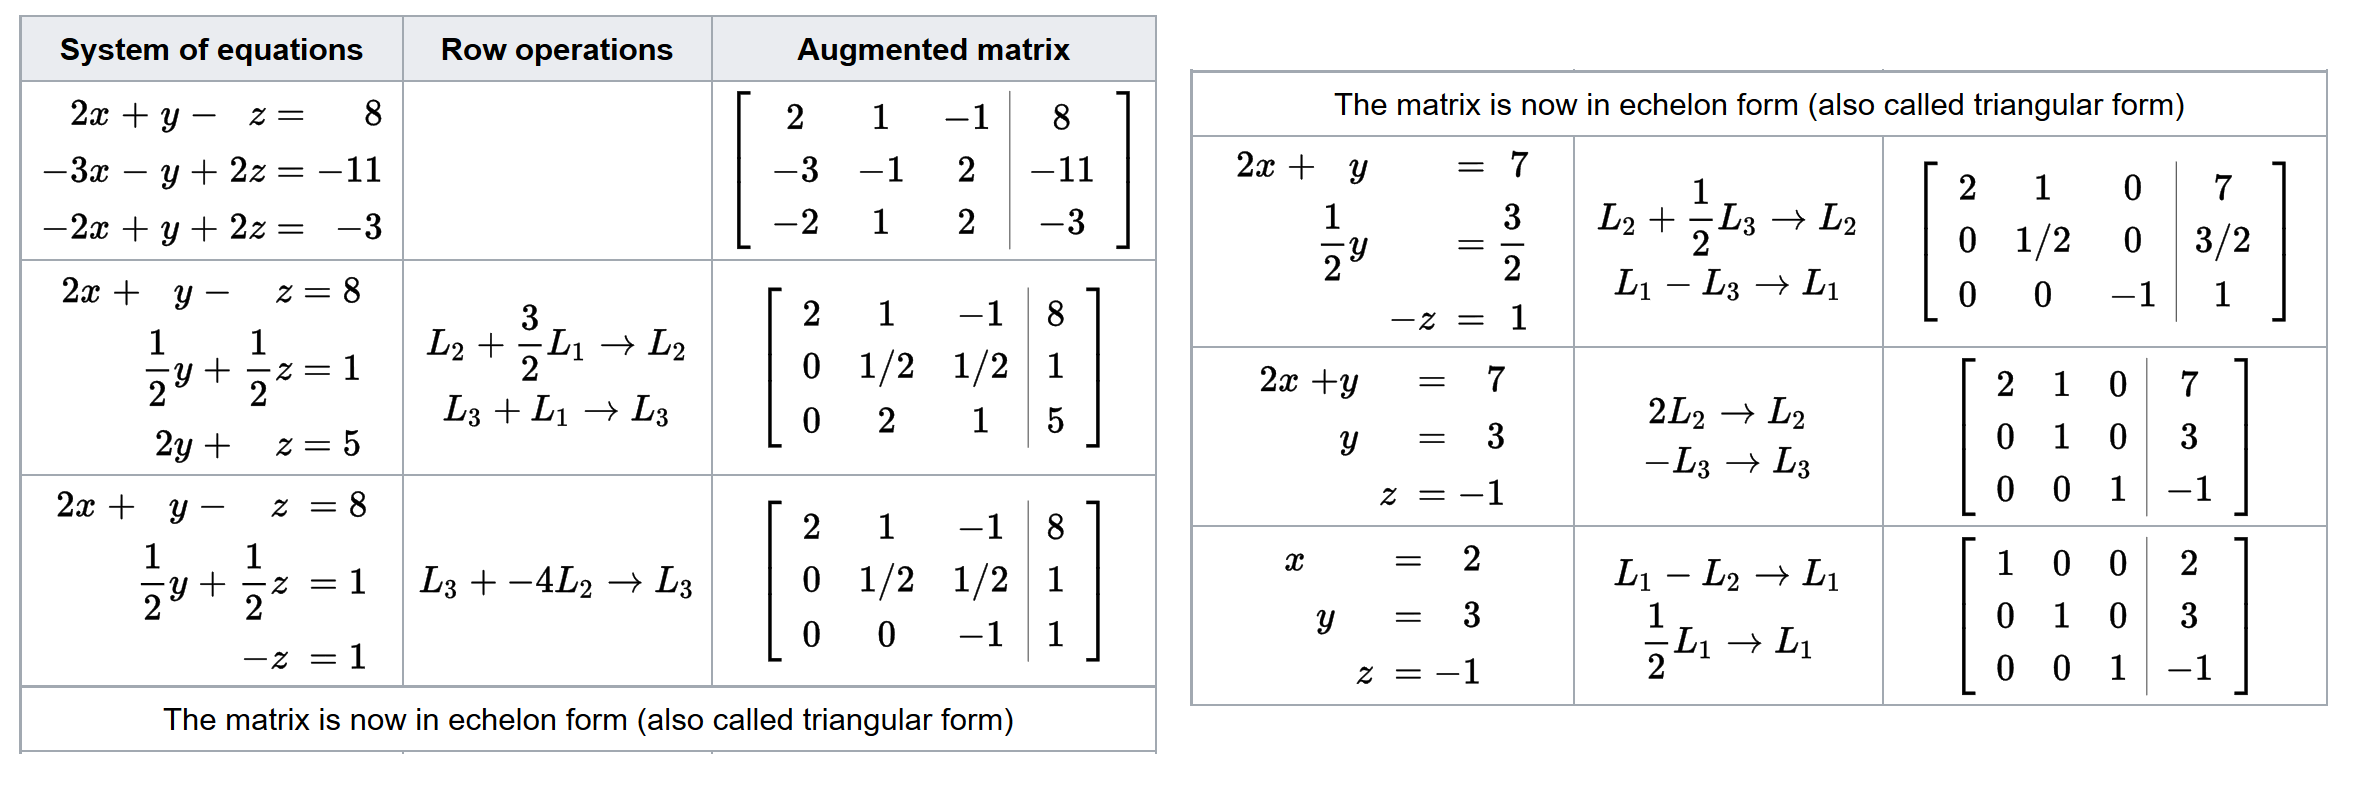
\includegraphics[width=\linewidth]{Images/gauss} 
\end{center}
\pause
\textbf{Practice: JSOI2008 sphere}
\end{frame}


%-------------------------------------------------------
\begin{frame}{Linear Algebra}
%-------------------------------------------------------
\textbf{Task: Given $n$ integers $\{a_1, a_2, ..., a_n\}$, select some s.t. the xor sum is maximum.} \\[0.5cm]
\pause
$n \leq 20$ ~ Brute-force search. \pause
~\\ That's definitely a terrible choice for $n \leq 100,000$. \\[0.5cm]
Hint: apply Gaussian elimination to the xor function. \\
\pause 
The time complexity is $O(n\log(MAX))$
\end{frame}

%-------------------------------------------------------
\begin{frame}{Linear Algebra}
%-------------------------------------------------------
\textbf{Practice Time} \\[0.5cm]
Given $n$ integers $\{a_1, a_2, ..., a_n\}, n\leq 100,000$. \pause
\begin{itemize}
	\item Select some, s.t. they have the minimum xor sum. \pause
	\item Select some, s.t. they have the maximum/minimum xor sum after appending another given integer $a$. \pause
	\item Select some, s.t. their xor sum is another given integer $a$. \pause
	\item Select one, s.t. it has maximum xor result with another given integer $a$, multiple queries (up to $100,000$).
\end{itemize}
\end{frame}

%-------------------------------------------------------
\section{Probability and Expectation}

%-------------------------------------------------------
\begin{frame}{Probability and Expectation}
%-------------------------------------------------------
\textbf{Probability}\\ 
Probability is the measure of the likelihood that an event will occur. \\[0.5cm]
\pause
\textbf{Expected value} \\ 
Expected value of a random variable, intuitively, is the long-run average value of repetitions of the experiment it represents.
$$E[X] = \sum_{k\in K} x_kP(k)$$
where $K$ is the set consists of all the events, $P(k)$ is the probability of event $k$.
\end{frame}

%-------------------------------------------------------
\begin{frame}{Probability and Expectation}
%-------------------------------------------------------
\textbf{Example} \\[0.5cm]
Let $X$ represent the outcome of a roll of a fair six-sided die. More specifically, $X$ will be the number of pips showing on the top face of the die after the toss. The possible values for $X$ are $1, 2, 3, 4, 5$ and $6$, all equally likely (each having the probability of $\frac16$). The expectation of $X$ is
$$E[X] = 1\cdot \frac16 + 2\cdot \frac16 + 3\cdot \frac16 + 4\cdot \frac16 + 5\cdot \frac16 + 6\cdot \frac16 = 3.5$$
\end{frame}


%-------------------------------------------------------
\begin{frame}{Probability and Expectation}
%-------------------------------------------------------
\textbf{Practice: POJ2096} \\[0.5cm]
A system has $s$ sub-systems, and it may produce $n$ kinds of bug. Ivan finds out 1 bug everyday, and it belongs to one kind and one sub-system. The probability bug belongs to each sub-system and each kind are uniform. Output the expected days that Ivan finds bugs from every sub-system and every kind. \\[0.5cm]
\pause
Hint: $f[i][j]$ represents the expected remaining days when Ivan has found $i$ kinds of bugs from $j$ sub-system.
\end{frame}


\section{Combinatorics}



\section{Introduction to Calculus}
\subsection{Differential of a Function}
\subsection{Calculus}

%-------------------------------------------------------



{\1
\begin{frame}[plain,noframenumbering]
  \finalpage{Part 2 ends here. Thank you for attention! \\ Powereed by \LaTeX. }
\end{frame}}

\end{document}